\chapter{Histograma de orientação de gradientes para poses de mão em um ambiente automotivo}

Esse capítulo tem como objetivo descrever as etapas da pesquisa prática. Conforme figura \ref{fig:research_steps} os principais passos do projeto são a construção da câmera infra vermelha, a geração da base de dados, a seleção das imagens que servirão de treinamento para o classificador SVM e depois o cálculo do HOG em todas as imagens variando os seus parâmetros e medindo o desempenho do algoritmo.

\begin{figure}[ht!]
	\centering
  	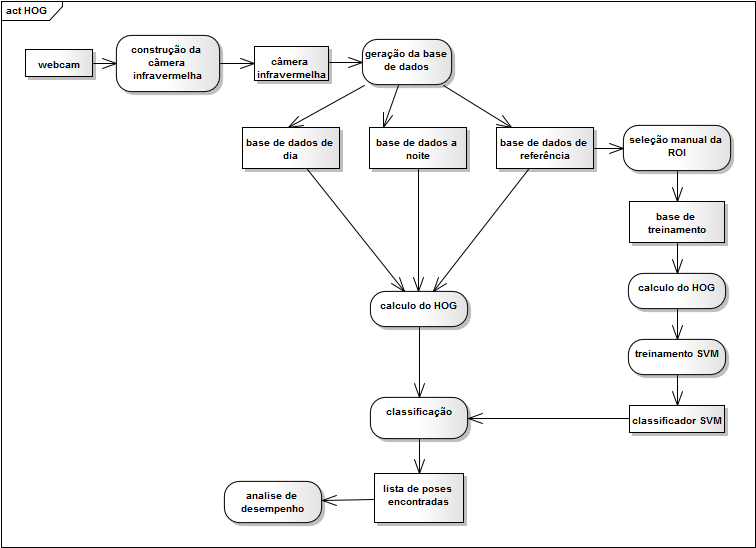
\includegraphics[scale=0.6]{image/HOG.png}
  	\caption{Fluxo de trabalho da pesquisa}
  	\label{fig:research_steps}
\end{figure}

\section{Construção da câmera infra vermelha}

A câmera utilizada nessa aplicação tem que ser capaz de capturar imagens nas mais diversas condições de luminosidade. Temos o caso, por exemplo, de um dia de sol cuja intensidade de luz é bem alta. Até o ponto onde não há luz nenhuma.
Nesses casos é necessário uma iluminação própria, mas ao mesmo tempo, não pode atrapalhar o motorista. Por isso, a iluminação infra vermelha é muito utilizada. O custo é baixo e não interfere em nada no ambiente. O maior contratempo desse tipo de iluminação é que se perde toda a informação de cor.
Para gerar a base de dados para o nosso estudo, utilizamos uma câmera normal de mercado, modificada para receber a luz infra vermelha e colocamos LEDs de infra vermelho para fazer a iluminação.

\begin{figure}[ht!]
	\centering
	\setlength{\fboxsep}{1pt}
	\fbox{
  		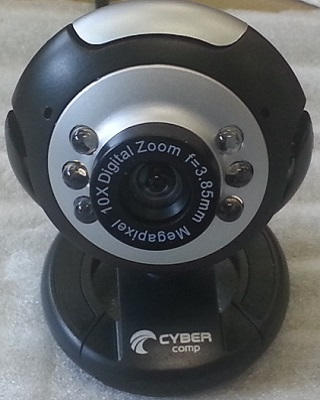
\includegraphics[scale=0.3]{image/webcam01.jpg}
 		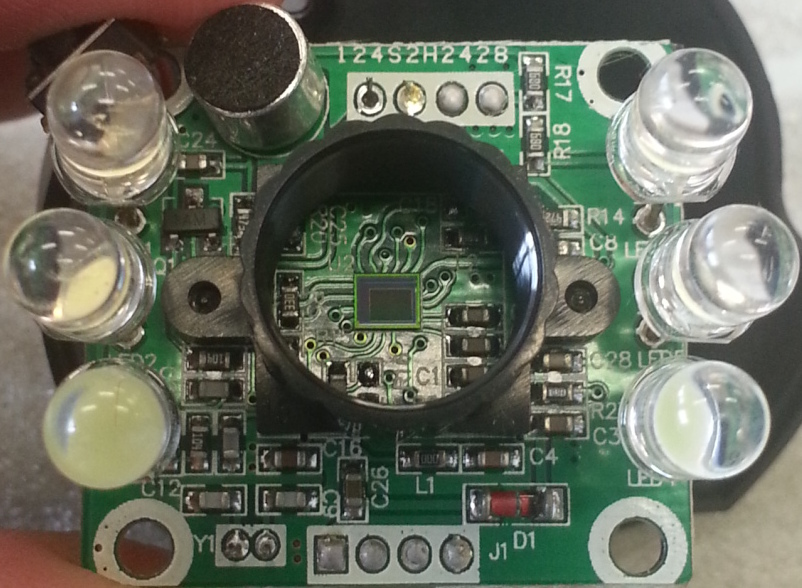
\includegraphics[scale=0.3]{image/webcam02.jpg}
 	}
  	\caption{Webcam utilizada na aquisição das imagens sem nenhuma modificação}
  	\label{fig:camera_01}
\end{figure}


Na figura \ref{fig:camera_01} temos a câmera utilizada para a aquisição das imagens. Nesse momento a câmera ainda não foi modificada. Essa câmera portanto ainda possui um filtro de luz infra vermelha e os LEDs de iluminação são LEDs brancos.

A principal modificação a ser feita nesse tipo de câmera é retirar o filtro infra vermelho. Esse filtro é uma placa de vidro localizado atrás da lente. Na figura \ref{fig:camera_02} temos uma foto das lentes ainda com o filtro e depois já com o filtro retirado. E preciso também substituir os LEDs atuais, que são LEDs brancos, para LEDs infra vermelho de 950nm.

\begin{figure}[ht!]
	\centering
	\setlength{\fboxsep}{1pt}
	\fbox{
		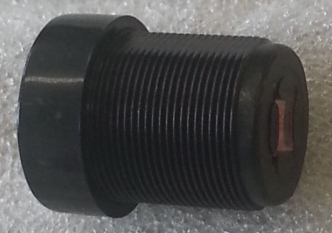
\includegraphics[width=0.3\textwidth]{image/webcam03.jpg}
  		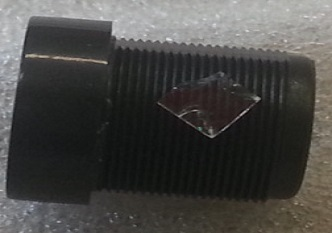
\includegraphics[width=0.3\textwidth]{image/webcam05.jpg}
  	}
  	\caption{Lentes com o filtro infra vermelho localizado na parte traseira}
  	\label{fig:camera_02}
\end{figure}

\section{Elaboração da base de dados}

As bases de dados que serão usadas no trabalho precisam refletir as condições que encontramos em um ambiente automotivo. Por isso elaboramos um conjunto de banco de imagens que variam o fundo, o usuário, a iluminação e a vestimenta. A resolução das imagens será 320x240 e a janela terá o tamanho de 120x110 pixels.

O nosso fundo vai variar conforme o carro aonde as imagens foram coletadas. Como referência, temos também um conjunto de imagens com o fundo preto homogêneo.
O usuário será também modificado, variando sexo e cor de pele. A iluminação terá a captura diurna e noturna e a vestimenta varia por exemplo se o usuário esta usando blusa, relógio, etc.

Para o usuário temos a tabela \ref{table:usuarios} mostrando as principais características dos mesmos.

\begin{table}[h]
	\centering
	\begin{tabular}{|c|c|c|}
		\hline Usuário & Sexo & Cor de pele \\
		\hline 1 & Masculino & Branco \\
		\hline 2 & Masculino & Branco \\
		\hline 3 & Feminino & Branco \\
		\hline 4 & Masculino & Moreno \\
		\hline 5 & Feminino & Negra \\
		\hline
	\end{tabular}
	\caption{Lista de usuários}
	\label{table:usuarios}
\end{table}

A nossa base de referência será uma banco de imagens com o fundo preto homogêneo, o usuário 1 do sexo masculino sem nenhum tipo de vestimenta ou acessório e a iluminação apenas dos LEDs infra vermelho, ou seja, em um ambiente totalmente escuro. Na tabela \ref{table:data_base_1} temos um resumo da parametrização dessa base e alguns exemplos das imagens.

\newcommand{\adddb}[9]{
\begin{table}[H]
	\centering
	\begin{tabular}{c c}
	\begin{tabular}{|c|c|}
		\hline \textbf{Usuário} 	& #1	\\ 
		\hline \textbf{Fundo} 		& #2	\\ 
		\hline \textbf{Iluminação} 	& #3	\\
		\hline \textbf{Vestimenta} 	& #4	\\
		\hline 
	\end{tabular} 
	&
	\begin{tabular}{|c|c|c|}
		\hline 
			\multicolumn{3}{|c|}{Gestos} \\ 
		\hline
			\raisebox{-.5\height}{\includegraphics[scale=0.3]{#5}} & 
			\raisebox{-.5\height}{\includegraphics[scale=0.3]{#6}} & 
			\raisebox{-.5\height}{\includegraphics[scale=0.3]{#7}} \\ 
		\hline 
	\end{tabular}
	\\
	\end{tabular}

	\caption{#8}
	\label{#9}
\end{table}
}

\adddb{Usuário 1}{Preto homogêneo}{Infra vermelha}{Nenhuma}{image/ir_led_1/0_02.jpg}{image/ir_led_1/1_02.jpg}{image/ir_led_1/7_02.jpg}{Parametrização da base de referência}{table:data_base_1}

% ***********************************************

Na tabela \ref{table:data_base_2} temos um conjunto de imagens com o fundo do carro Ford Focus, iluminação com LEDs infra vermelhos e usuário 1 com uma blusa preta.

\adddb{Usuário 1}{Ford Focus}{Infra vermelha}{Blusa preta}{image/night/focus/gustavo/blackshirt/0_02.jpg}{image/night/focus/gustavo/blackshirt/1_01.jpg}{image/night/focus/gustavo/blackshirt/7_01.jpg}{Parametrização do conjunto 2}{table:data_base_2}

% ***********************************************

Na tabela \ref{table:data_base_3} temos um conjunto de imagens com o fundo do carro Ford Focus, iluminação com LEDs infra vermelhos e usuário 1 sem vestimentas.

\adddb{Usuário 1}{Ford Focus}{Infra vermelha}{Nenhuma}{image/night/focus/gustavo/shortshirt/0_02.jpg}{image/night/focus/gustavo/shortshirt/1_01.jpg}{image/night/focus/gustavo/shortshirt/7_01.jpg}{Parametrização do conjunto 3}{table:data_base_3}

% ***********************************************

Na tabela \ref{table:data_base_4} temos um conjunto de imagens com o fundo do carro Passat, iluminação com LEDs infra vermelhos e usuário 2 usando uma blusa verde. O interessante desse conjunto é a existência de um LED no painel que pode atrapalhar a segmentação da imagem.

\adddb{Usuário 2}{Passat}{Infra vermelha}{Blusa verde}{image/night/passat/rogerio/blusaverde/0_02.jpg}{image/night/passat/rogerio/blusaverde/1_01.jpg}{image/night/passat/rogerio/blusaverde/7_01.jpg}{Parametrização do conjunto 4}{table:data_base_4}

\section{Desenvolvimento da Pesquisa}

Como vimos anteriormente na tabela \ref{table:dlal_hog}, o HOG é calculado usando células de 8x8 pixeis, agrupas em blocos de 2x2 células. Portanto se aplicarmos o HOG com os parâmetros originais em uma imagem de 320x240, teremos 40x30 células. Cada célula contribui duas vezes para a formação do vetor de características por conta na sobreposição que existe na normalização em blocos, com exceção das bordas, que contribuem apenas uma vez. Portando teremos 40 + (40-2) x 30 + (30-2) células. Cada histograma tem 9 grupos de ângulos totalizando um vetor de 40.716 dimensões. Na figura \ref{fig:hog_example1} temos um exemplo visual do HOG. Cada histograma de cada célula é mostrado usando um diagrama de rosa. O tamanho de cada pétala do diagrama é ajustado para indicar a contribuição que aquela orientação representa no histograma da célula. 

\begin{figure}[ht!]
\centering
\fbox{
  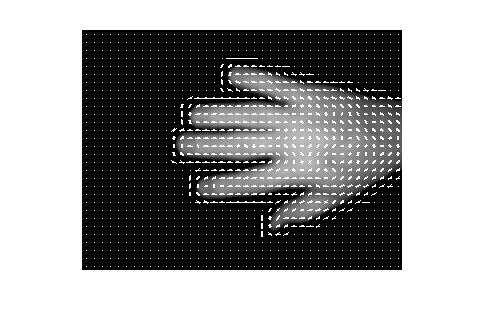
\includegraphics[scale=0.7]{image/hog/0_01.png}
  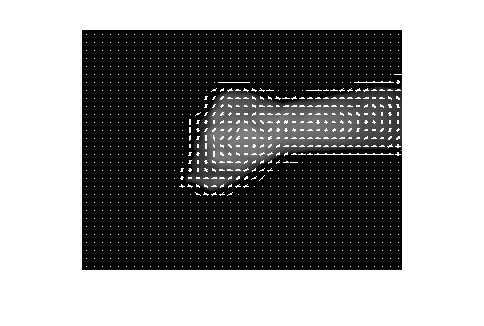
\includegraphics[scale=0.7]{image/hog/7_01.png}}
  \caption{Exemplos do cálculo do HOG com os parâmetros originais}
  \label{fig:hog_example1}
\end{figure}

\subsection{Implementação do HOG}

Em construção.

\subsection{Resultados}

Para quantificar a performance dos classificadores que serão criados, optou-se pela geração de um gráfico do tipo DET (Detection Error Tradeoff). Esse tipo de gráfico é usado em classificações binárias medindo falso negativo vs. falso positivo em uma escala log-log. As curvas de gráficos do tipo DET tendem a ser mais lineares do que as curvas ROC (Receiver Operating Characteristics), facilitando a análise para pequenas variações. Os eixos serão: Taxa de Erro (\(FalsoNeg/VerdadeiroPos + FalsoNeg\)) versus Falso Positivo por Janela (FPPW do inglês False Positive per Window).

Primeiramente será criado um conjunto de classificadores para cada pose de mão que a pesquisa abrange. Esse conjunto é formado por 3 classificadores com foco na variação da luminosidade. Um para as imagens feitas durante o dia, um outro para as imagens infra vermelhas feitas à noite e um terceiro que seria genérico tanto para dia quanto para noite. O intuito é testar se a performance de um classificador específico para a luminosidade é melhor do que um classificador que abrange os dois tipos.

As imagens de treinamento serão geradas manualmente extraindo uma janela (110x120) com a pose de mão correspondente da base de referência. 

Cada classificador será avaliado considerando imagens da pose versus imagens sem a pose e depois imagens da pose versus imagens de outras poses. Esse teste permite avaliar quais as poses são mais parecidas.

Considerando que temos 10 poses diferentes, teremos um total de 30 classificadores.
 
Depois um novo conjunto de classificadores será gerado (um para cada tipo de luminosidade) mas com treinamento de todas as poses com o objetivo de detectar mão independente da pose.

Esse conjunto de testes será repetido para cada parâmetro do cálculo do HOG conforme tabela \ref{table:hog_var}.

\begin{table}[H]
	\centering
		\begin{tabular}{|c|c|}
		\hline  
			Número de células 		&  8x8 até 240x240 		\\ 
		\hline  
			Número de blocos  		&  2x2 e 1x1 			\\ 
		\hline 
			Tipo de normalização  	&  L2-norm, L2-Hys,  L1-norm , L1-sqrt 										\\ 
		\hline 
			Agrupamento dos ângulos	&  9 a 36				\\ 
		\hline
			Sinal dos ângulos		& 0-180 / 0-360			\\
		\hline		
		\end{tabular} 
		\label{table:hog_var}
\end{table}

O tempo de cálculo será medido para cada parâmetro avaliado, para que depois se possa analisar o quão mais rápido o algoritmo se torna conforme seu desempenho cai.

\chapter{Discussão}

O objetivo desse capítulo é discutir a relação entre a hipótese formulada no trabalho, a teoria existente sobre o assunto e a prática demonstrada no capítulo anterior.

\chapter{Conclusão}

Em construção.